
\section{Training details}
\label{sec:training}
\noindent We adopt in two stages to effectively learn dense perception capabilities. In the first stage, \textbf{Multi-Teacher Distillation}, we initialize the model weights by distilling knowledge from strong vision teachers (DINOv3 and SigLIP2) into our unified dense backbone. This provides a robust initialization for visual features. In the second stage, \textbf{Perception training}, we train the model on approximately 685 GT of multimodal data using our specialized "Chain-of-Perception" format (\texttt{<coord><size><seg>}). This stage fine-tunes the backbone and heads to perform autoregressive dense prediction tasks. We detail each stage and our design choices below.


\subsection{Multi-Teacher Distillation for Weights Initialization\label{sec:mtd}}

To help train our early-fusion perception models, we use the multi-teacher distillation pipeline described by~\citep{chaybouti2025amoe} to initialize the weights of the models. The motivation of this strategy is to benefit from the distinct strengths of diverse vision backbones: we use the ViT-H variant of DINOv3~\citep{simeoni2025dinov3} to inherit its strong local features, critical for our segmentation head; and SigLIP2-So400m~\citep{tschannen2025siglip} to inject knowledge and language-aligned features for open-vocabulary expression understanding.

\noindent We use this initialization on the two model scales: the 22-layer (300M parameters) and the 28-layer (600M parameters) dense models. The distillation is performed over the OpenLVD-200m~\citep{chaybouti2025amoe} dataset, supplemented by 9 million high-resolution scrapped images, 11 million images from the SAM~\citep{kirillov2023segment} dataset, and 5 million documents. Training consists of a single multi-resolution stage up to $1024 \times 1024$ pixels, spanning approximately \num{200}k steps. We use the Muon~\citep{jordan2024muon} optimizer. The training is distributed across four 8-A100 GPU nodes, employing sequence packing with a local batch size of 6 and a maximum sequence length of \num{4096} tokens to maximize computational throughput.

\noindent \textbf{Evaluation.} To assess the quality of the learned representations, we evaluate the models on standard vision benchmarks. For linear probing semantic segmentation tasks, we conduct a learning rate search and report the best mIoU obtained. As shown in Table~\ref{tab:distillation_results}, the multi-teacher distillation provides a strong foundation for both general classification and dense spatial tasks.

\begin{table}[t]
\centering
\caption{Performance of the two dense models initialized via multi-teacher distillation. All evaluations are run at $512\times512$ maximum number of pixels.\vspace{-0.2cm}}
\setlength{\tabcolsep}{6pt}
\adjustbox{width=\textwidth}{
\begin{tabular}{l c c c c c}
\toprule
\textbf{Model}  & \textbf{ImageNet-1k (zero-shot)} & \textbf{kNN} & \textbf{Cityscapes} & \textbf{Pascal VOC} & \textbf{ADE20K} \\
\midrule
22-layer & 70.84\% & 82.58\% & 60.77\% & 83.81\% & 48.10\% \\
28-layer & 74.25\% & 84.00\% & 62.72\% & 85.11\% & 49.10\% \\
\bottomrule
\end{tabular}
}
\label{tab:distillation_results}
\end{table}




\subsection{Data Curation}

\noindent We construct a large-scale, high-quality dataset of 54M images with 195M positive expressions, and 488M negatives ones, with a total of 570M masks through a multi-stage pipeline: 

\noindent \textit{Clustering $\to$ VLM Listing $\to$ Negative Mining $\to$ Ensemble Consensus $\to$ Human Verification}. This process ensures diversity of expressions and images, semantic granularity, and high-precision annotations.

\noindent \textbf{Seed Data via Hierarchical Clustering:}
Starting from a large pool of web-scraped images, we employ the hierarchical clustering and sampling technique to mitigate long-tail biases~\citep{vo2024automatic}. Specifically, we embed images using a DINOv3 ViT-B encoder and perform a 4-level hierarchical clustering (20M $\to$ 500k $\to$ 50k $\to$ 20k centroids). We then sample a balanced subset of \textit{54M diverse seed images}, ensuring broad and uniform concept coverage.

\noindent \textbf{Listing via VLM:}
We prompt a powerful  VLM to generate dense object listings for each image. Crucially, we instruct the VLM to categorize outputs according to our PBench complexity levels (Section~\ref{sec:complexity-levels}). The resulting distribution is heavily weighted towards foundational capabilities: 60\% of samples target Levels 0-1 (Objects \& Attributes), with the remaining 40\% spread across Levels 2-4 (OCR, Spatial, Relations).

\noindent \textbf{Negative Mining:}
To robustify the model against hallucinations, we generate hard negative queries for each image. We feed the image and its positive concepts back into the VLM to generate three types of negatives: (i) \textit{Semantic Negatives:} Concepts in the same category but absent (\eg, "sushi" vs. "pizza"); (ii) \textit{Visual Confounders:} Objects that look similar to present instances; and (iii) \textit{Hard Semantic Negatives:} Fine-grained distinctions (\eg, specific cat breeds).

\noindent \textbf{Annotation via Ensemble Consensus:}
We employ a multi-model agreement mechanism to generate high-quality synthetic  labels.
\begin{itemize}
    \item \textbf{Levels 0-1:} We use an ensemble of SAM 3, Qwen3-VL-30B, and Qwen3-VL-8B. For each sample, we randomly select a pair of models. A sample is accepted only if all matched the pair aligns with an IoU $> 0.8$.
    \item \textbf{Levels 2-4:} We use Qwen3-VL-30B, Moondream3, and Qwen3-VL-8B. Similarly, we require agreement between a randomly sampled pair. Since these are detection models, we convert agreed bounding boxes to segmentation masks using SAM 2.
\end{itemize}

The agreement algorithm uses Hungarian matching to align predictions and strictly enforces both count matching and high spatial overlap.

\noindent \textbf{Human Verification Loop:}
Disagreements are not discarded. We route the subset of non-agreed samples (approx. 4M) to human annotators for manual verification (Accept/Reject). Accepted samples are incorporated into the training mix, while rejected samples are then sent for full manual re-annotation from scratch. This loop recovers hard samples that confuse the automated ensemble, preventing the dataset from being biased towards "easy" consensus examples, and helps mine hard samples where most models fail.


\noindent \textbf{Public Datasets:} We supplement our curated data with: OpenImages~\citep{kuznetsova2020open}, Objects365~\citep{shao2019objects365}, WCS camera traps~\citep{lila_bc_wcscameratraps}, marine datasets~\citep{jansen2022underwater,saleh2020realistic,lila_bc_river_herring}, iSAID~\citep{waqas2019isaid}, Fashionpedia~\citep{jia2020fashionpedia}, iNaturalist-2017~\citep{van2017inaturalist} and VisDrone-Det~\citep{zhu2021detection}. For datasets with bounding boxes, we convert the annotations to masks using SAM-2~\citep{sam2}.

\noindent \textbf{Text only data:}
To enhance the language modeling capabilities of our unified backbone, we mix in high-quality text-only data during training. We utilize publicly available pre-training corpora and SFT datasets, such as Fineweb \citep{penedo2024fineweb}, to ensure the model develops general language abilities alongside the dense perception task.

\subsection{Design choices}
The aimed capabilities  introduce design challenges. We detail the key sweeps conducted to finalize the design. Settings for each experiment were kept constant across variants. For efficiency, we perform ablations only on the detection task, except for feature regularization, where segmentation is used to better analyze retention of high-quality image features. 

\noindent \textbf{Sequence format:} We serialize the task into a unified sequence format: 

\texttt{<image>expr$_1$<present><coord><size><seg>$\cdots$<eoq>expr$_2$<absent><eoq> $\cdots$ <eos>}. The end of query block is marked by \texttt{<eoq>}. We introduce explicit \texttt{<present>} and \texttt{<absent>} tokens immediately following the text expression to impose a strong inductive bias: the model must explicitly commit to a binary decision about the object's existence \textit{before} attempting any localization. 

\noindent \textbf{Configuration:} We train a 600M parameter model for Falcon Perception. Images are processed at a maximum resolution of $1024 \times 1024$ with a patch size of 16, ensuring high-fidelity visual encoding. This base configuration remains consistent across all stages, with specific adaptations to learning rates and masking strategies as detailed below.


\noindent \textbf{(\textit{i}) Loss Balancing across Ranks:}
In our multimodal training with packed sequences, the number of valid tokens varies significantly across ranks due to varying sizes of the images, number of expressions and instances per packed sample. We identified that standard FSDP gradient averaging biases the loss towards ranks with fewer tokens. We implemented a global normalization strategy where the loss is first aggregated across the ranks and then scaled by the \textit{global} average number of tokens ($N_{total}/R$) rather than the local rank count. Details in \ref{sec:loss}.

\noindent \textbf{(\textit{ii})  Optimizer Choice - Muon \vs AdamW:}
We observed that the specialized heads (Coordinates, Size, Segmentation) often lagged behind the language backbone during training. We compared standard \textit{AdamW} against \textit{Muon} (a momentum-based optimizer) for these heads to balance learning rates between the pre-trained backbone and initialized perception modules. Fig.~\ref{fig:optim} shows the training loss comparison between Muon and AdamW optimizer for the language, coord and size heads. We observe that employing the Muon optimizer leads to lower training losses across the different heads, yielding improved performance on both PBench and SaCo benchmarks in terms of macroF1 (Tab.~\ref{tab:optim}). 
\begin{figure}[t]
\centering
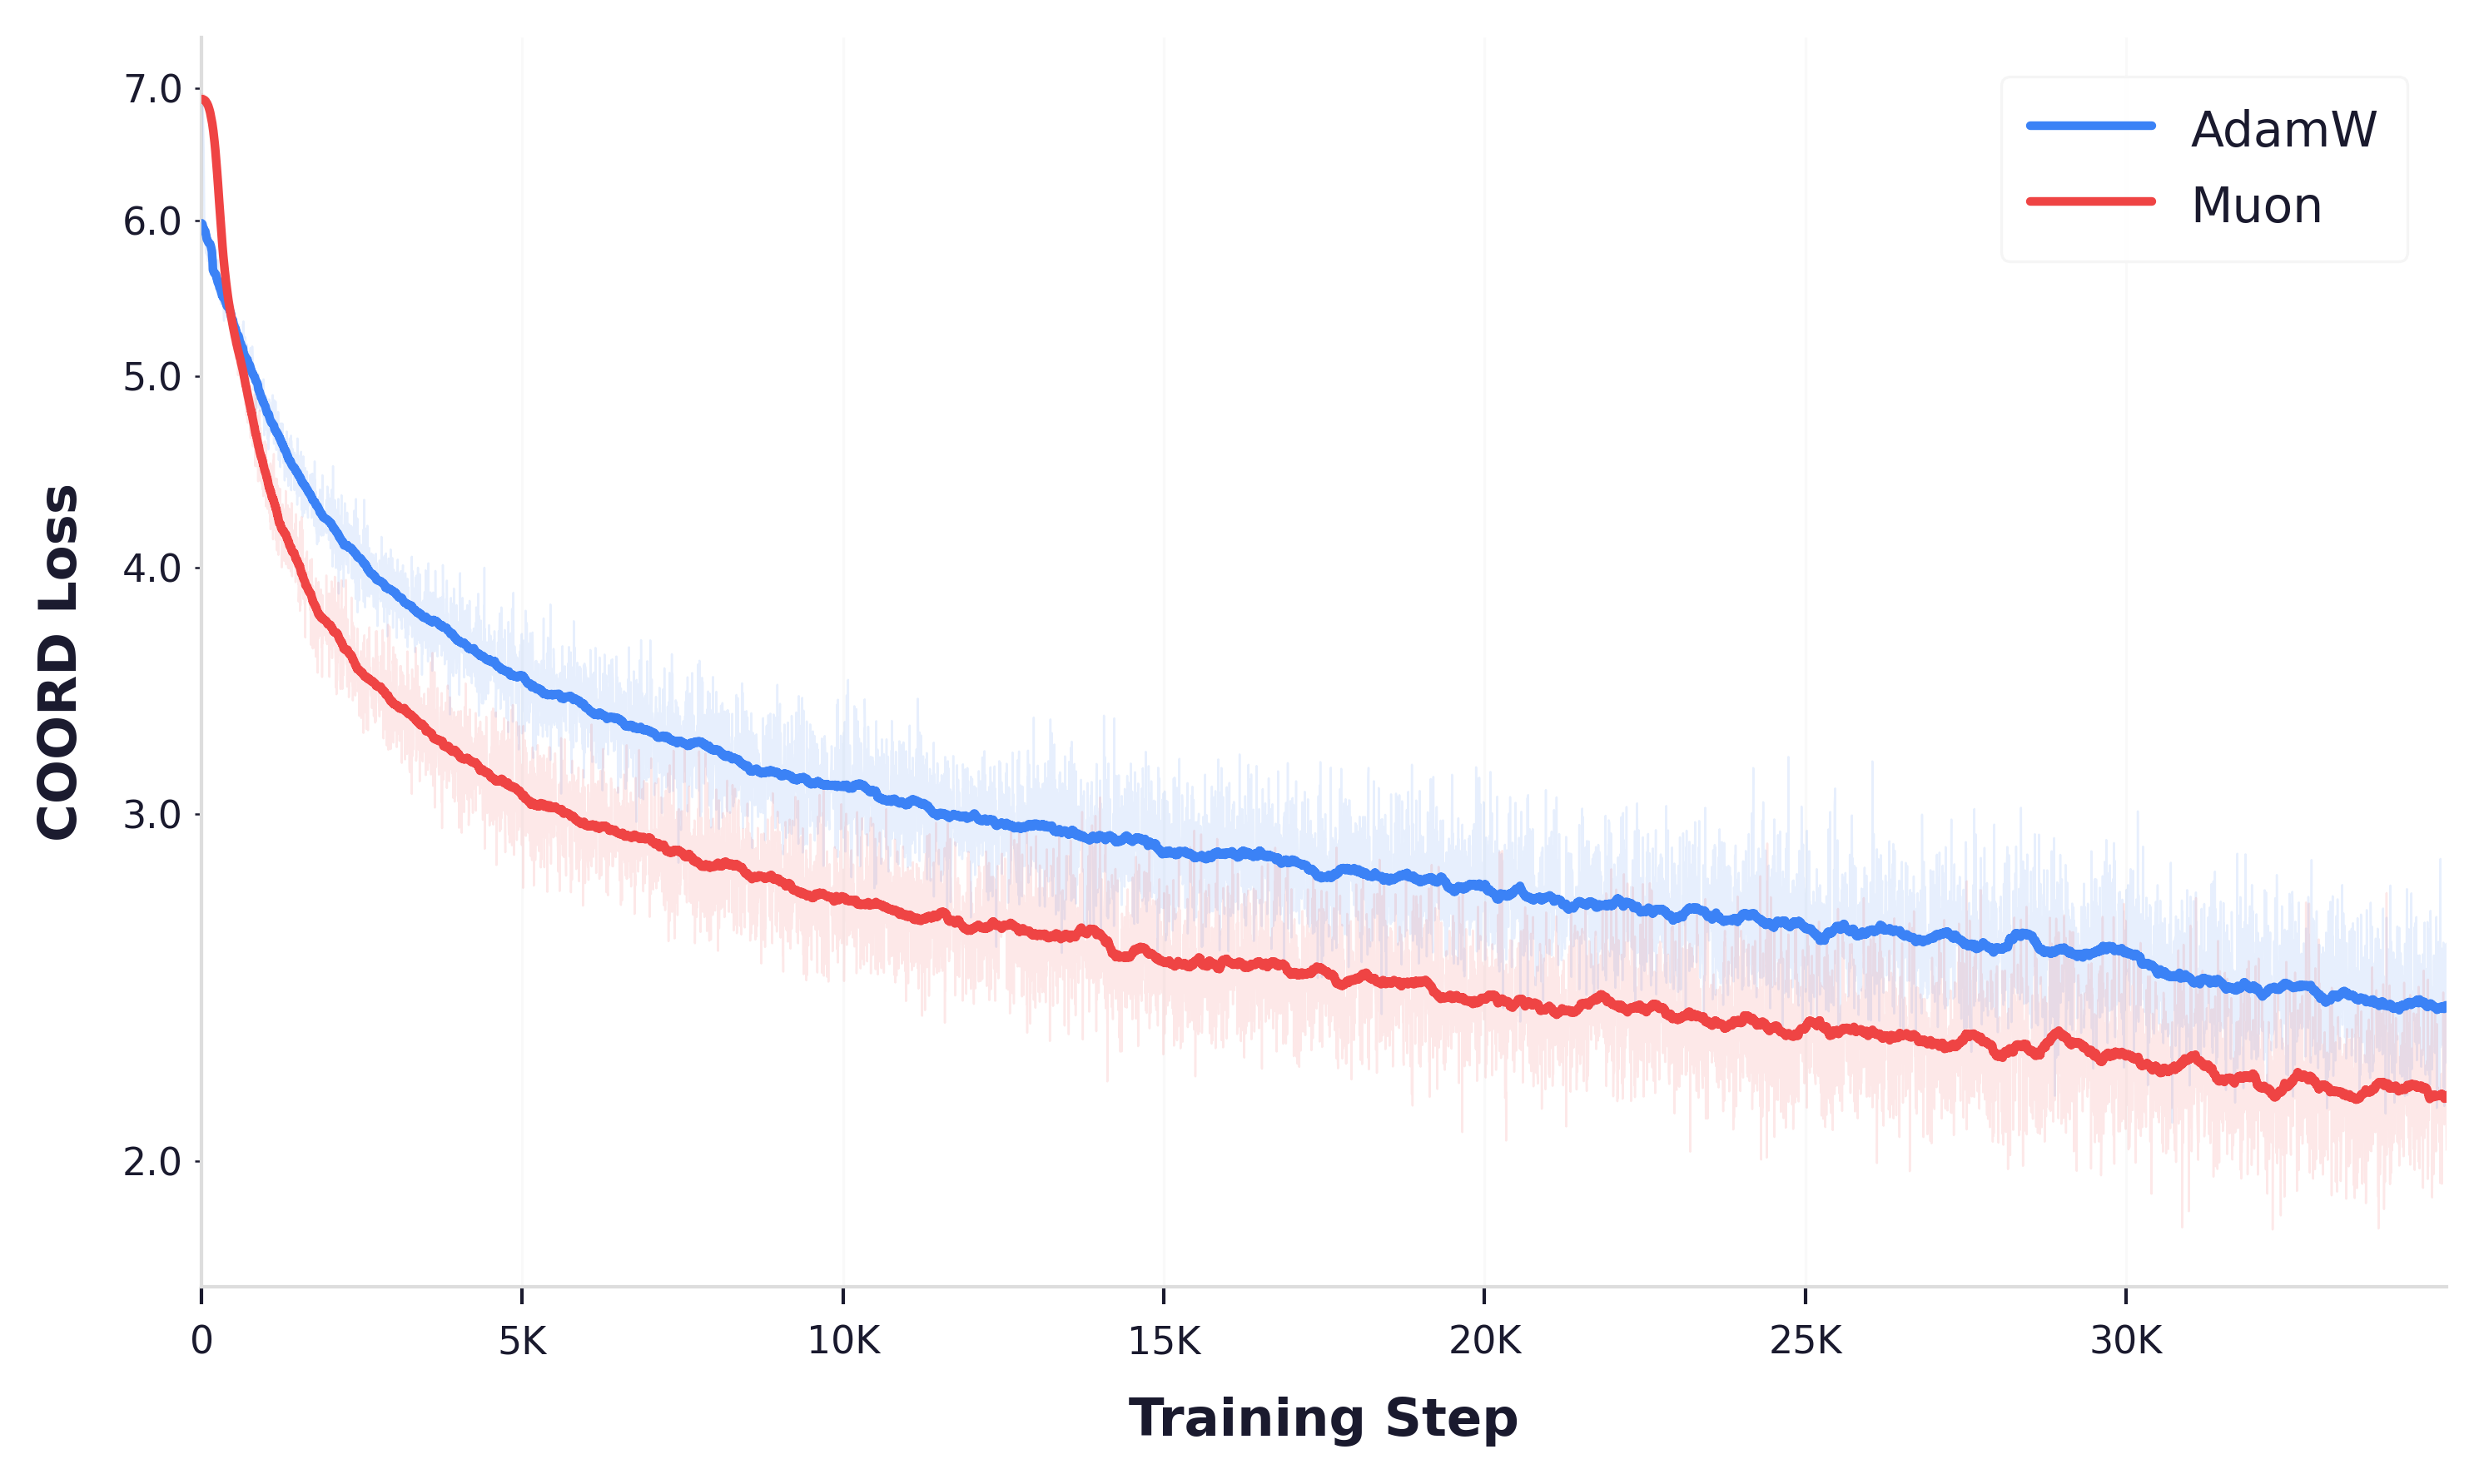
\includegraphics[width=0.33\linewidth]{figures/sweeps/optim_coord}
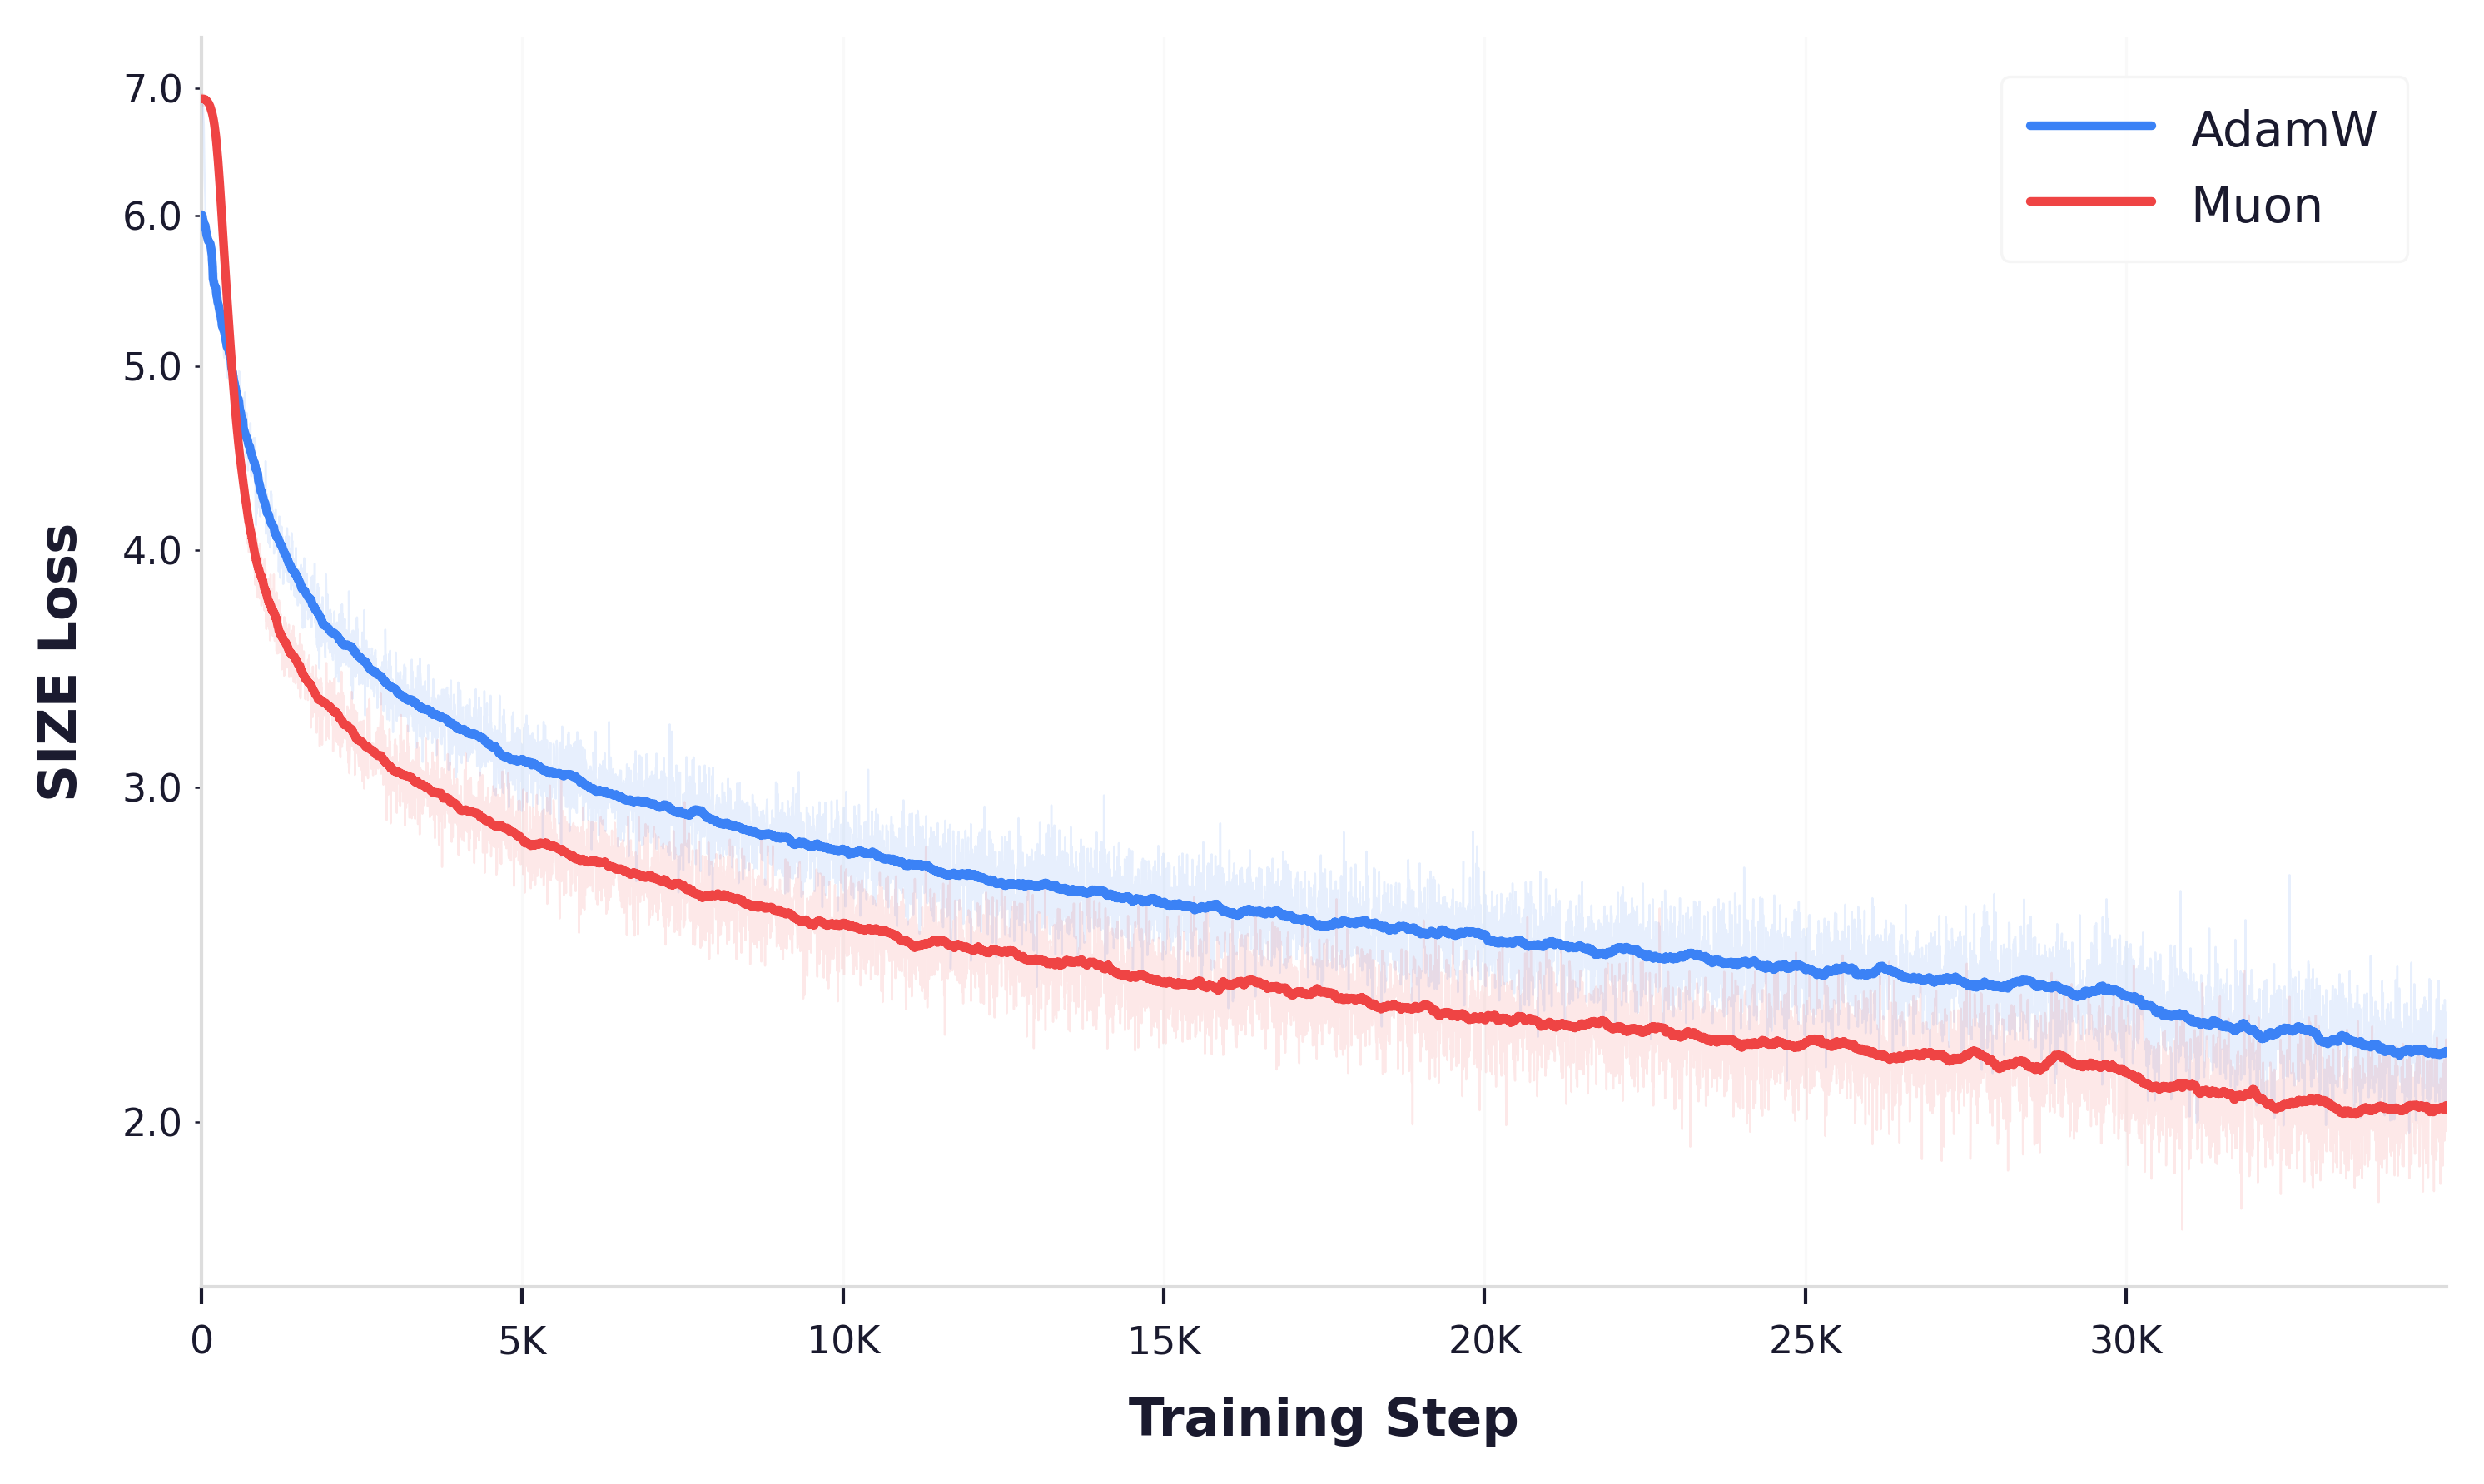
\includegraphics[width=0.32\linewidth]{figures/sweeps/optim_size}
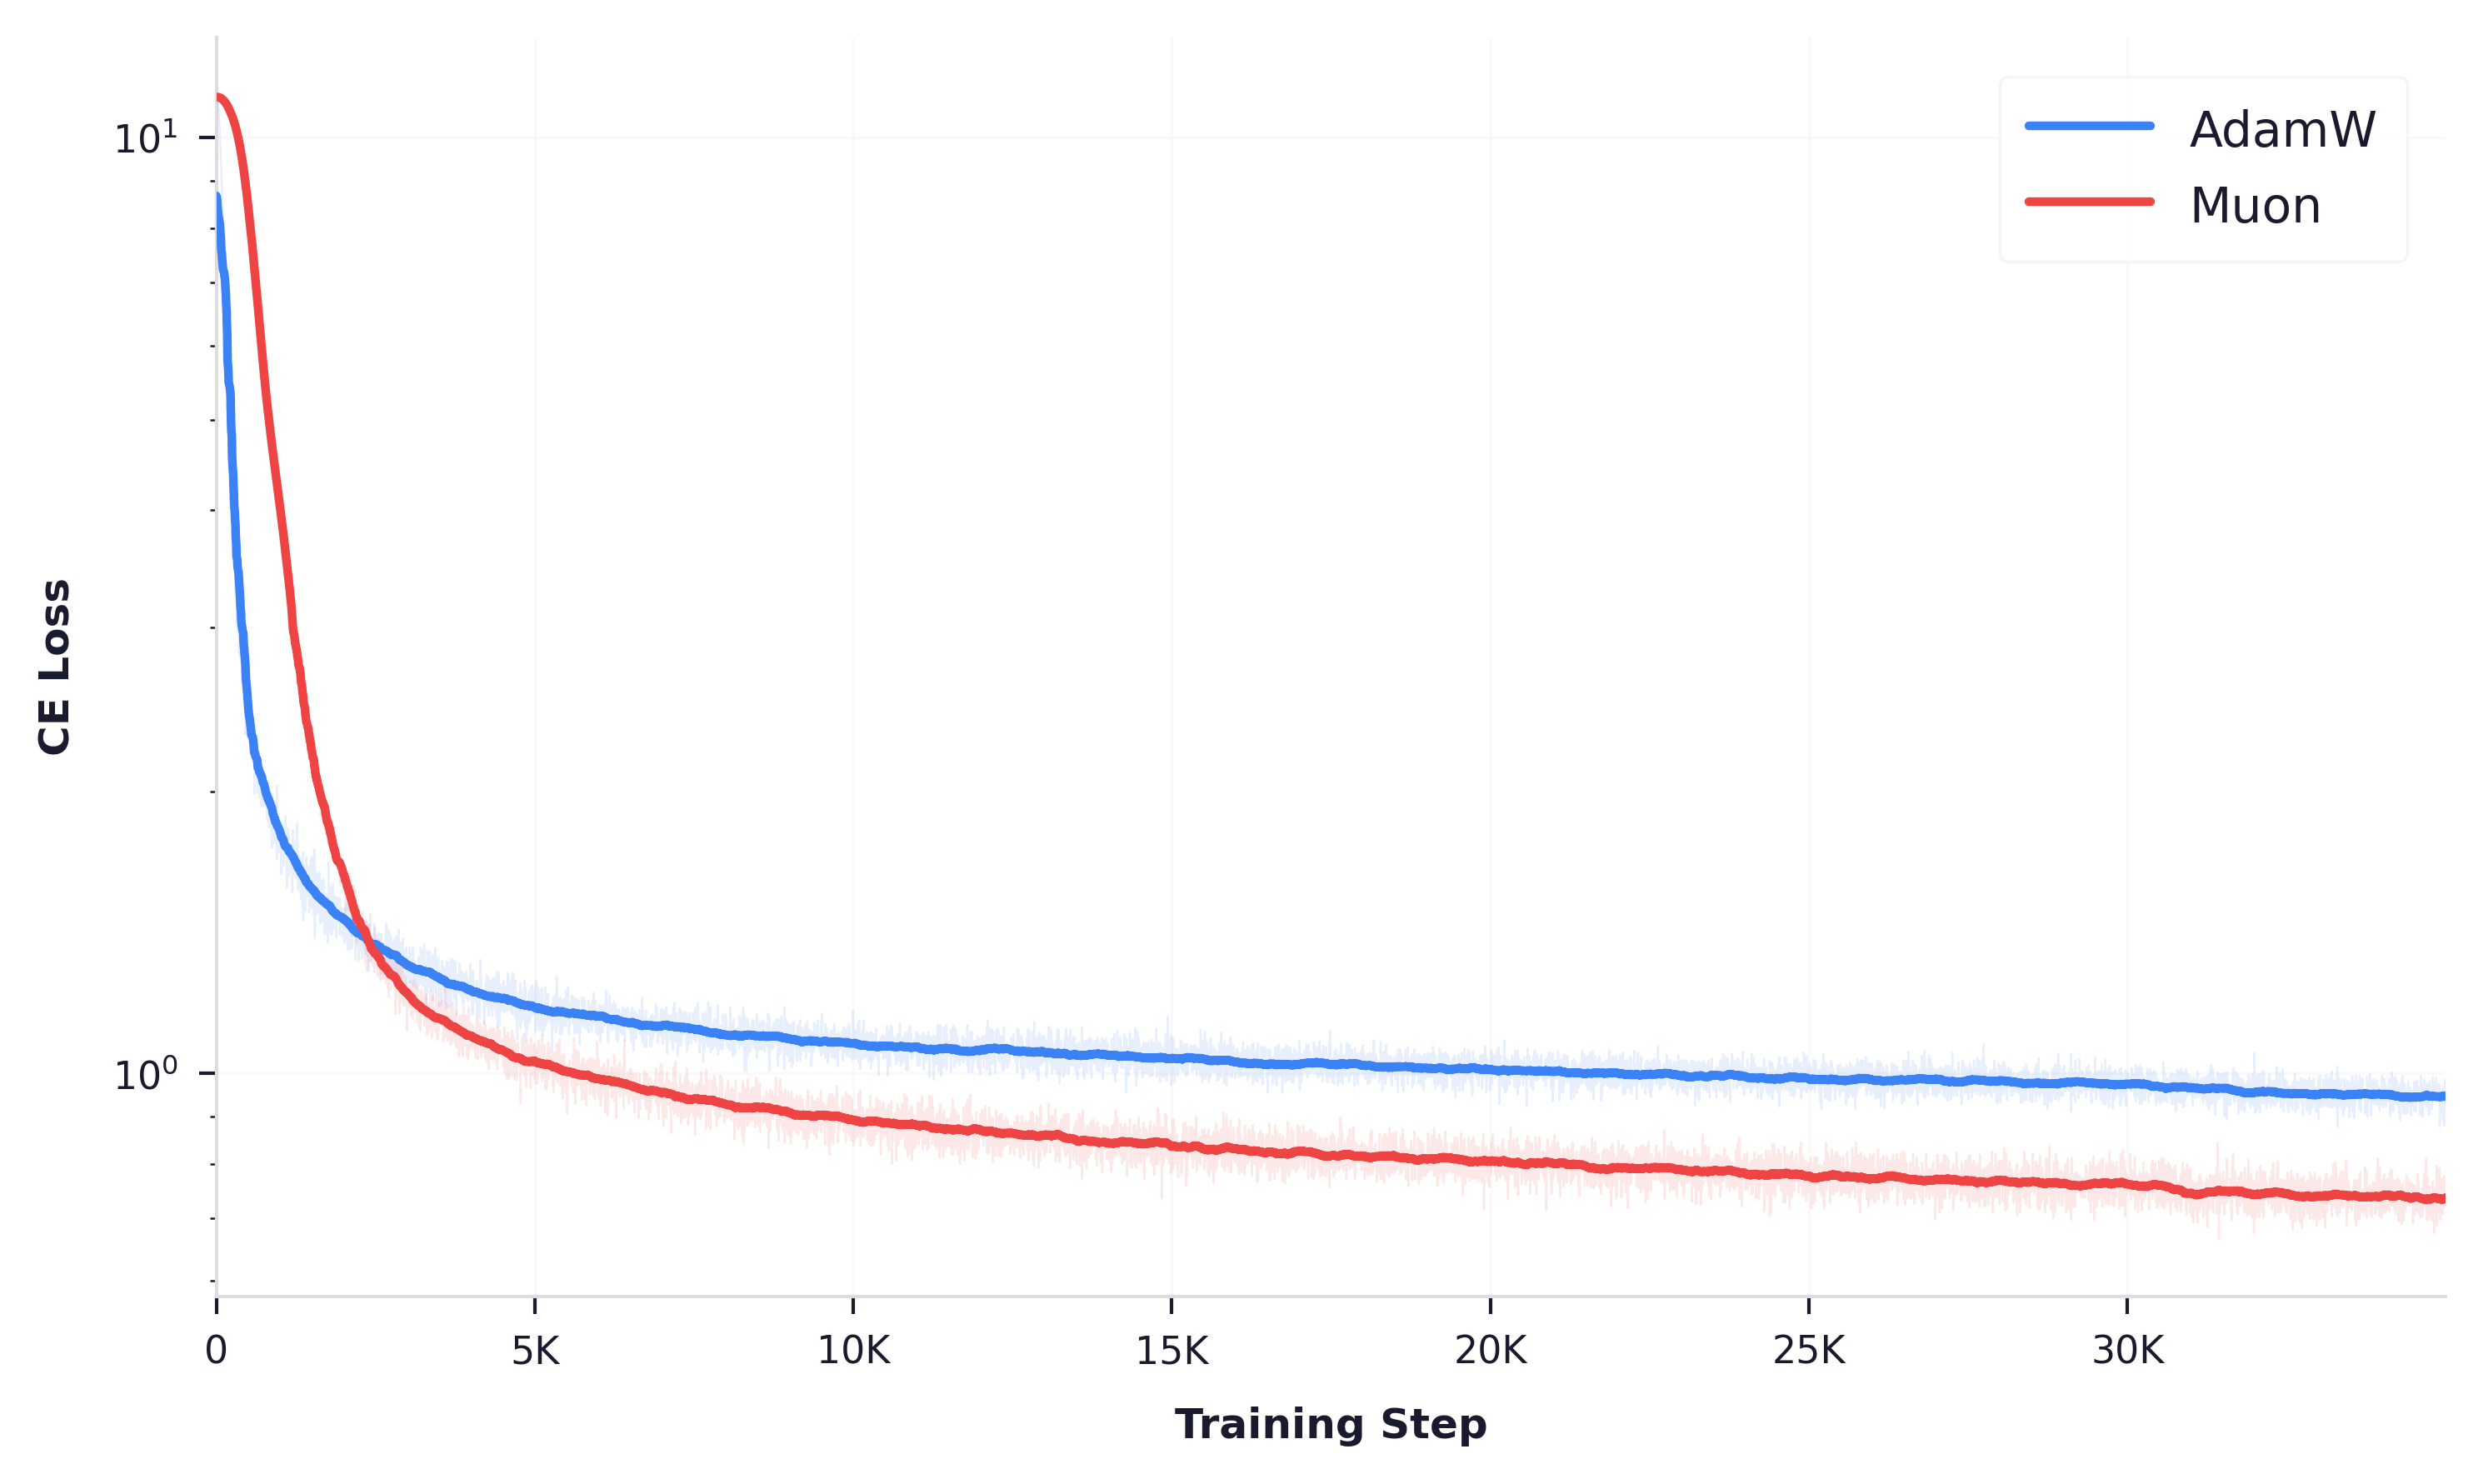
\includegraphics[width=0.32\linewidth]{figures/sweeps/optim_ce}
\caption{Muon optimizer results in lower training losses for coord, size and cross-entropy, in comparison to AdamW, leading to improved performance (Tab.~\ref{tab:optim}).\label{fig:optim}}
\end{figure}



\noindent \textbf{(\textit{iii}) Feature Regularization (Gram Loss):}
We introduce the Gram loss, similar to DINOv3~\citep{simeoni2025dinov3}, as a regularization to maintain the structural integrity of the visual feature space. This enforces that the correlation matrix (Gram matrix) of the student's patch features matches that of a frozen teacher model. From the ablation experiment in Tab.~\ref{tab:gram}, we observe that training with the Gram loss indeed results in better performance on both benchmarks since it enables better image feature retention that is required for the segmenting the instances, compared to learning the task without the Gram regularization. 


\noindent \textbf{(\textit{iv}) Attention and Causality:}
We investigated the attention mechanism between queries.
\textit{Full AR \vs No Inter-query Attn:} We compared full causal attention (where queries attend to the image features in addition to the previous queries and their corresponding instances) against a masked approach, where queries attend to the image but not to each other, assessing the trade-off between relational reasoning and computational efficiency. Full AR enables in-context learning among the queries, where the model can learn to skip predicting the positions occupied by instances from previous queries. In contrast, the inter-query masking attention forces the model to focus on the image content to predict the instances for a particular query. Although the ablation in Tab.~\ref{tab:querymask} shows a marginal advantage for the query masking variant, since both the strategies rely on complimentary information for prediction, we employ them both in different stages of our model training, as detailed in Sec.~\ref{sec:recipe}. 
\begin{table}[t!]
\begin{minipage}{0.32\textwidth}
    \centering
    \setlength{\tabcolsep}{4pt}
    \captionof{table}{AdamW \vs Muon\vspace{-0.2cm}}
    \label{tab:optim}
    \adjustbox{width=0.95\columnwidth}{
    \begin{tabular}{c|cc}
        \toprule
         \textbf{Optimizer} & \textbf{PBench-\textit{Det}} & \textbf{SaCo-\textit{Det}} \\
         \midrule
         AdamW & 56.4 & 49.0 \\
         Muon & 57.7 & 53.8 \\
        \bottomrule
        
    \end{tabular}
    }

\end{minipage}
\begin{minipage}{0.32\textwidth}
    \centering
    \setlength{\tabcolsep}{4pt}
    \captionof{table}{Impact of Gram Loss\vspace{-0.2cm}}
    \label{tab:gram}
    \adjustbox{width=0.95\columnwidth}{
    \begin{tabular}{c|cc}
        \toprule
         \textbf{Feature Reg.} & \textbf{PBench-\textit{Seg}} & \textbf{SaCo-\textit{Seg}} \\
         \midrule
         No Gram & 52.7 & 51.1 \\
         With Gram & 53.8 & 52.6 \\
        \bottomrule
    \end{tabular}
    }
\end{minipage}
\begin{minipage}{0.33\textwidth}
    \centering
    \setlength{\tabcolsep}{4pt}
    \captionof{table}{Inter-query Masking\vspace{-0.2cm}\label{tab:querymask}}
    \adjustbox{width=0.95\columnwidth}{
    \begin{tabular}{c|cc}
        \toprule
         \textbf{Ordering} & \textbf{PBench-\textit{Det}} & \textbf{SaCo-\textit{Det}} \\
         \midrule
         Full AR & 53.2 & 53.1 \\
         Query Masking & 54.2 & 53.3 \\
        \bottomrule
    \end{tabular}
    }
    
\end{minipage}


\end{table}

\noindent \textbf{(\textit{v}) Mask Ordering:}
When multiple objects are present, the order of target sequences matters. We compared between \textit{random}, \textit{size} (largest instance to smallest) and \textit{raster} ordering. We observe that raster ordering converges faster to a lower loss for the coord head among the three variants (Fig.~\ref{fig:ordering}). We hypothesize that raster is better since it enables our model to search for objects in a clear order (which is not possible for the other two variants) and learn faster with lesser ambiguity. And since the coordinate token is predicted first for an instance, lower coord loss (\ie, a better learned coord head) directly translates to an improved detection performance in terms of macroF$_1$ on both PBench and SaCo benchmarks.


\noindent \textbf{(\textit{vi}) Sequence format:} 
Since segmentation masks are highly expressive and bounding boxes can be trivially extracted from them, it is natural to ask why we utilize the \texttt{<coord><size><seg>} sequence rather than simply predicting \texttt{<seg>}. We justify our design choice based on two primary factors: (i) When trained solely on \texttt{<seg>}, the model defaults to predicting a merged semantic mask for all instances. Resolving this would require integrating an expensive segmentation mask encoder. Instead, we use a lightweight \texttt{<coord>} encoder; conditioning the \texttt{<seg>} prediction on these bounding boxes natively enables distinct instance masks. (ii) Generating \texttt{<seg>} requires invoking the upsampling module. Our sequence formulation allows the model to operate as a pure object detector by simply not decoding the \texttt{<seg>} token, bypassing the upsampling module entirely for faster inference.

\begin{figure}[h]
\centering

\begin{minipage}{0.6\textwidth}
    \centering
    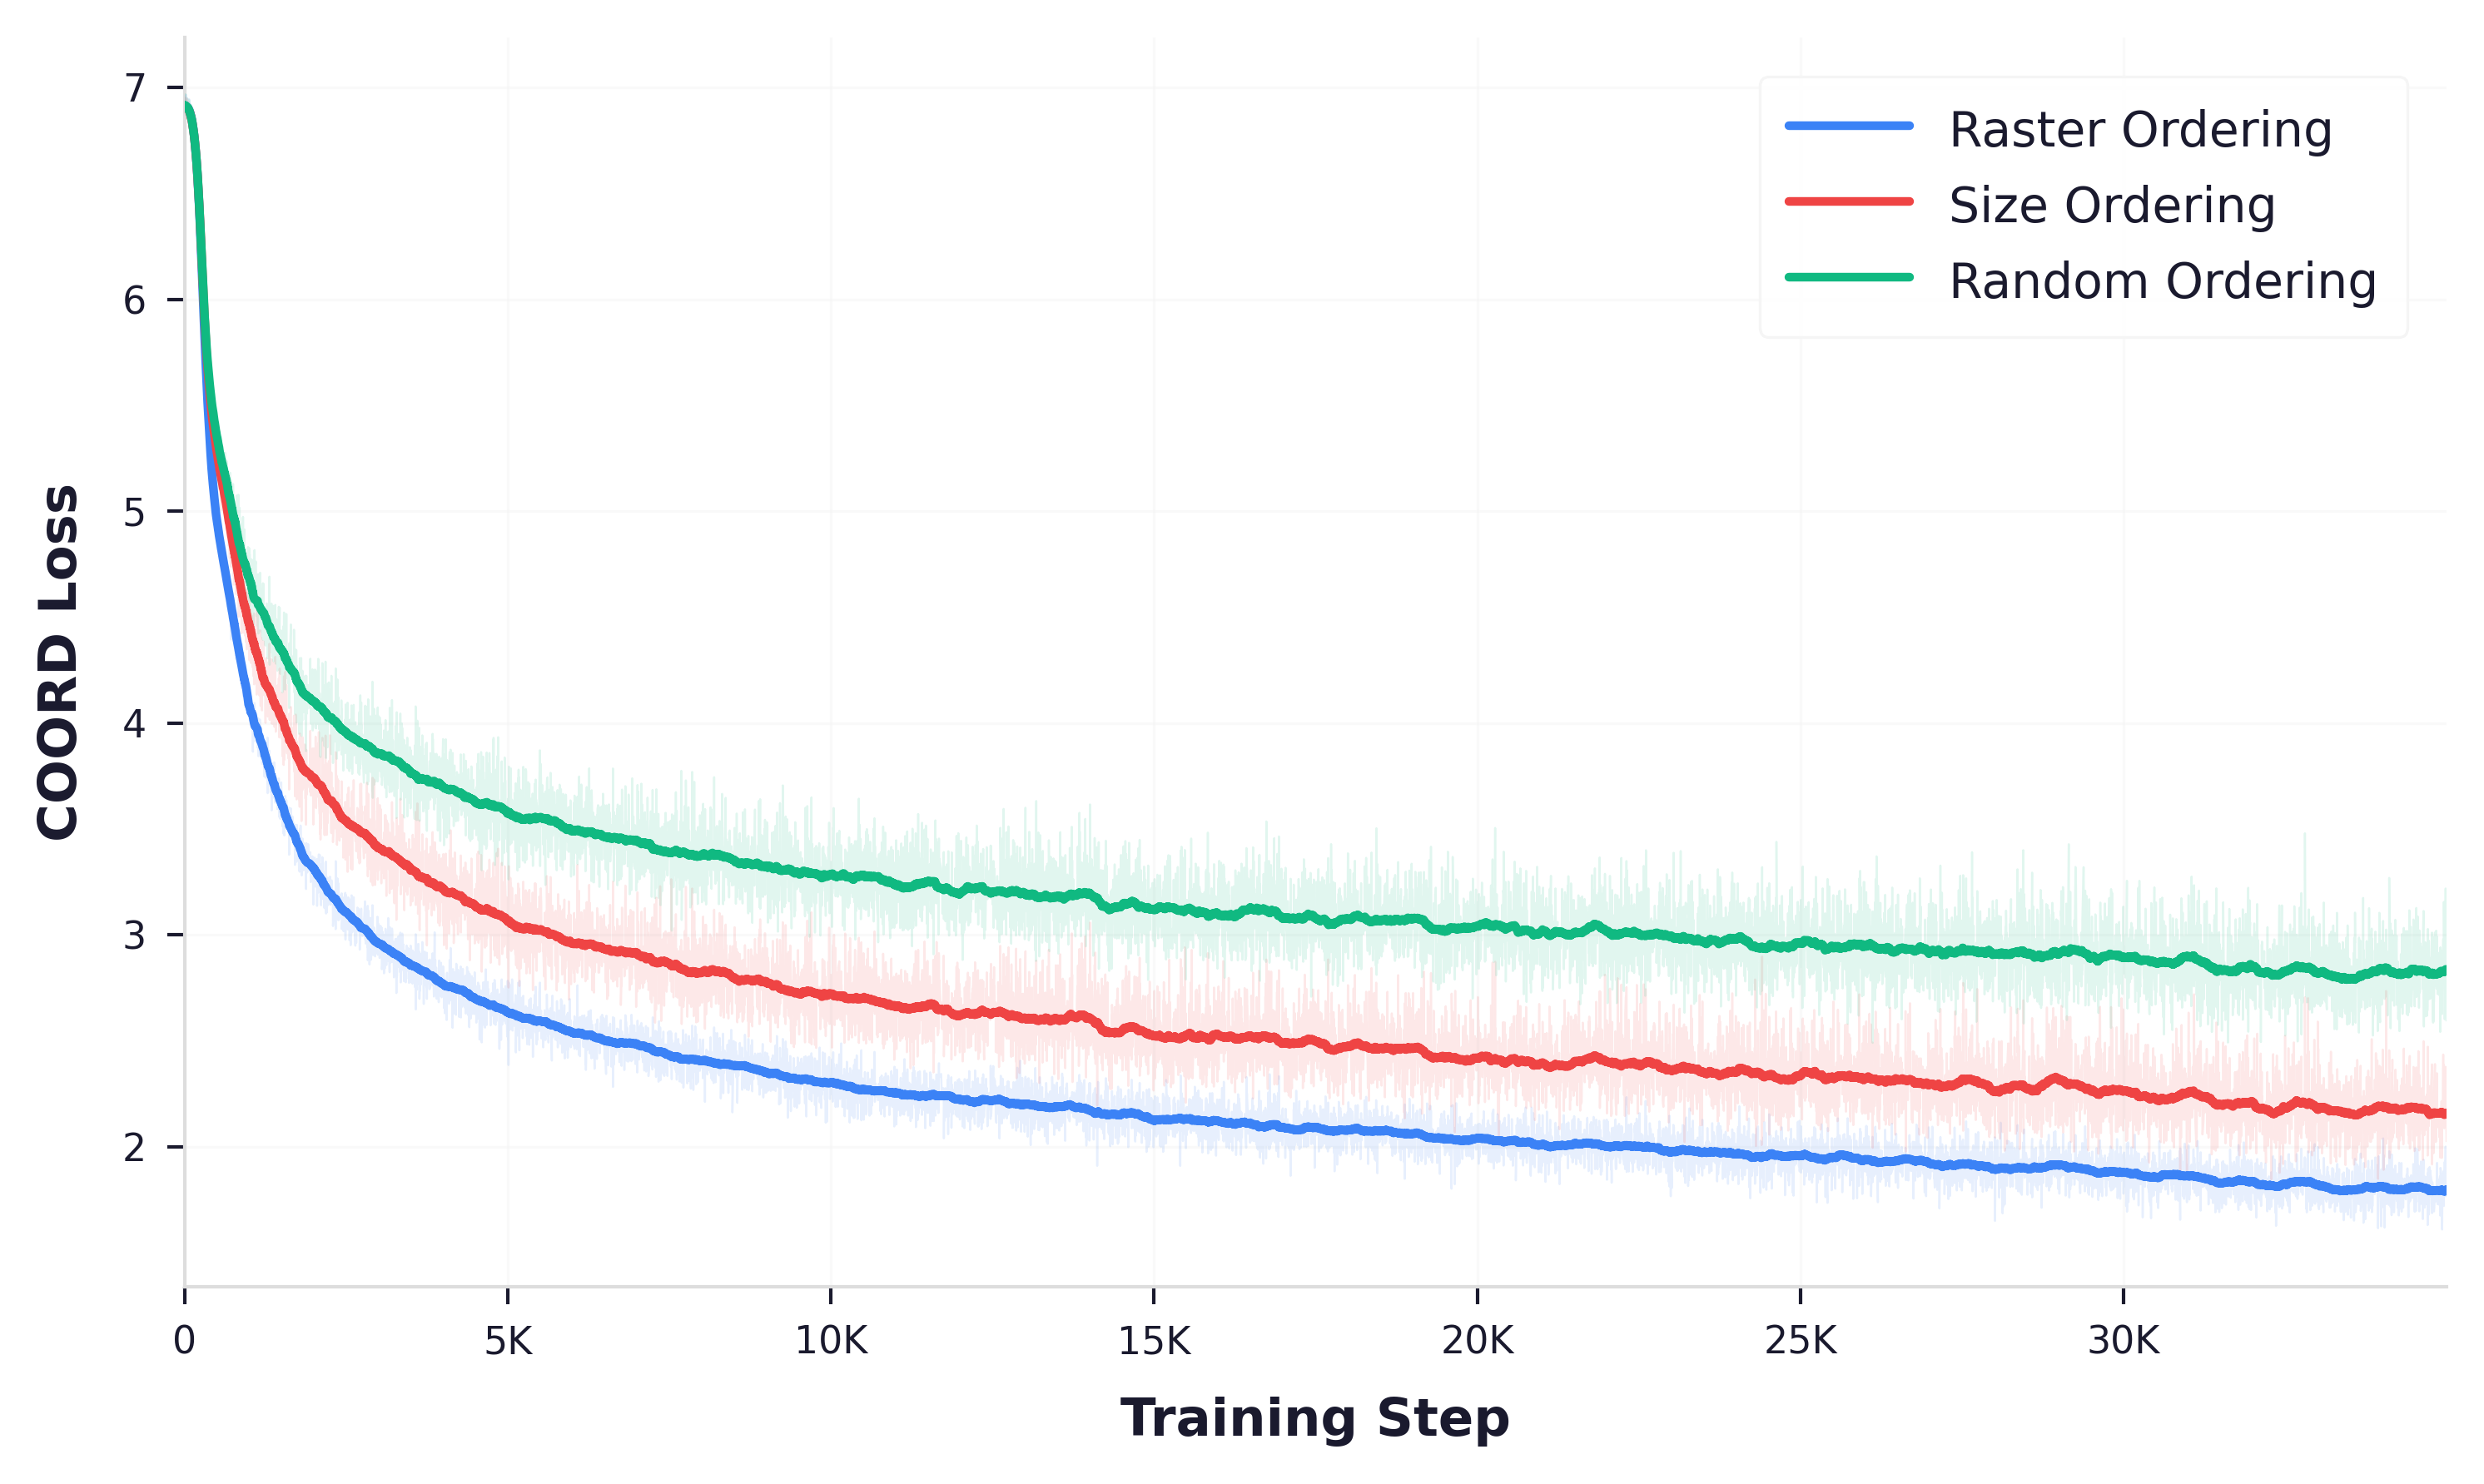
\includegraphics[width=\linewidth]{figures/sweeps/order_coord}
\end{minipage}
\hfill
\begin{minipage}{0.39\textwidth}
    \centering
    \setlength{\tabcolsep}{5pt}
    \adjustbox{width=0.9\columnwidth}{
    \begin{tabular}{c|cc}
        \toprule
         \textbf{Ordering} & \textbf{PBench-\textit{Det}} & \textbf{SaCo-\textit{Det}} \\
         \midrule
         Random & 52.2 & 46.3 \\
         Size & 57.7 & 53.8 \\
         Raster & 59.3 & 56.2 \\
        \bottomrule
        
    \end{tabular}
    }
   
\end{minipage}

\caption{Raster ordering of instances results in lower training loss and better performance on both benchmarks, compared to random and size orderings.\label{fig:ordering}}

\end{figure}


\subsection{Objective functions}
\label{sec:loss}

\noindent We train Falcon Perception with a weighted sum of language modeling, structured geometry, dense mask, and feature-alignment losses. Each object is $O_k=(c_k,s_k,m_k)$ with center $c_k\in[0,1]^2$, size $s_k\in[0,1]^2$, and binary mask $m_k\in\{0,1\}^{H\times W}$. Coordinate/size/mask supervision is applied \emph{only} for the positive (present) queries, while absent (negative) queries contribute only through the language modeling loss.

\noindent \textbf{Language modeling loss:}
Let $X$ be the unified sequence and let $p_\theta(x_i\mid x_{<i},I)$ be the backbone next-token distribution. We compute cross-entropy on non-ignored tokens and normalize by the \emph{global} average number of valid tokens across data-parallel ranks to avoid bias from variable numbers of ignored tokens (\eg, due to variable image token counts):
\begin{equation}
\mathcal{L}_{\text{lm}} \;=\; \frac{\sum_{i:\,y_i\neq \texttt{IGNORE}} -\log p_\theta(y_i \mid X_{<i})}{\max(1,\;\overline{N}_{\text{text}})}\,,
\end{equation}
where $\overline{N}_{\text{text}}$ denotes the average number of valid text/task labels per loss-rank.

\noindent \textbf{Coordinate loss:}
The coordinate head predicts discrete bins with $B=1024$ bins per axis. We discretize ground-truth coordinates by
\begin{equation}
q(c) \;=\; \mathrm{clip}\!\Big(\mathrm{round}\big(c\cdot(B-1)\big),\;0,\;B-1\Big)\,,
\end{equation}
applied elementwise to $c_k=(c^x_k,c^y_k)$. Let $\ell^c_k\in\mathbb{R}^{2\times B}$ be the coordinate logits from the coordinate head. The loss is
\begin{equation}
\mathcal{L}_{\text{coord}} \;=\; \frac{1}{\max(1,\overline{N}_{\text{coord}})}\sum_{k\in\mathcal{K}^+}\sum_{a\in\{x,y\}}
\mathrm{CE}\!\left(\ell^{c,a}_k,\; q(c^a_k)\right),
\end{equation}
where $\mathcal{K}^+$ is the set of positive objects and $\overline{N}_{\text{coord}}$ is the global-average count of supervised coordinate targets.

\noindent \textbf{Size loss (log-scale binning):}
Size is supervised on a log scale to allocate more resolution to small objects. With $B=1024$ bins and $s_k=(s^w_k,s^h_k)$, we clamp and map to a normalized log space:
\begin{equation}
\tilde{s} \;=\; \frac{\log_2(\max(s,\;1/B)) - \log_2(1/B)}{0-\log_2(1/B)} \in [0,1]\,,
\qquad
q_s(s) \;=\; \mathrm{round}\big(\tilde{s}\cdot(B-1)\big)\,.
\end{equation}
Let $\ell^s_k\in\mathbb{R}^{2\times B}$ be size logits. We use
\begin{equation}
\mathcal{L}_{\text{size}} \;=\; \frac{1}{\max(1,\overline{N}_{\text{size}})}\sum_{k\in\mathcal{K}^+}\sum_{a\in\{w,h\}}
\mathrm{CE}\!\left(\ell^{s,a}_k,\; \mathrm{clip}(q_s(s^a_k),0,B-1)\right).
\end{equation}

\noindent \textbf{Mask losses (focal + dice):}
Given predicted mask logits $\hat{m}_k\in\mathbb{R}^{H\times W}$ (Equation~(4) in Section~\ref{sec:heads}) and ground-truth mask $m_k$, we use a weighted focal loss and a dice loss:
\begin{equation}
\mathcal{L}_{\text{seg}} \;=\; \beta\,\mathcal{L}_{\text{focal}} \;+\; \alpha\,\mathcal{L}_{\text{dice}},
\qquad \alpha=10,\;\beta=200,
\end{equation}
with normalization by the global-average number of supervised masks $\overline{N}_{\text{seg}}$:
\begin{equation}
\mathcal{L}_{\text{focal}} \;=\; \frac{1}{\max(1,\overline{N}_{\text{seg}})}\sum_{k\in\mathcal{K}^+}\mathrm{Focal}(\hat{m}_k,m_k),
\qquad
\mathcal{L}_{\text{dice}} \;=\; \frac{1}{\max(1,\overline{N}_{\text{seg}})}\sum_{k\in\mathcal{K}^+}\mathrm{Dice}(\hat{m}_k,m_k).
\end{equation}

\noindent \textbf{Gram feature alignment:}
To prevent loosing the image features from the distillation phase, we add a Gram loss between student and teacher patch features (when available). Let $F_s,F_t\in\mathbb{R}^{N\times d}$ denote (normalized) student/teacher visual features for the $N$ valid patches, and let $M\in\{0,1\}^{N}$ be the valid-patch mask. Define Gram matrices $G_s=F_sF_s^\top$ and $G_t=F_tF_t^\top$, and mask out invalid patch pairs. The loss is
\begin{equation}
\mathcal{L}_{\text{gram}} \;=\; \frac{\| (G_s-G_t)\odot (MM^\top)\|_F^2}{\max(1,\langle MM^\top, \mathbf{1}\rangle)}.
\end{equation}

\noindent \textbf{Final objective:}
Putting everything together, the final training objective is given by
\begin{equation}
\mathcal{L} \;=\; \mathcal{L}_{\text{lm}} \;+\; \mathcal{L}_{\text{coord}} \;+\; \mathcal{L}_{\text{size}} \;+\; \mathcal{L}_{\text{seg}} \;+\; \lambda_{\text{gram}}\mathcal{L}_{\text{gram}}\,,
\qquad
\lambda_{\text{gram}}=0.1.
\end{equation}

\subsection{Training Recipe\label{sec:recipe}}

Following the multi-teacher distillation, we train the model on the perception task for a total of approximately 685 Gigatokens (GT). We adopt  three stages  designed to first build a robust, globally-aware scene understanding, and subsequently specialize the model for the independent query task required at inference time. Throughout all stages, we strictly maintain a 1:1 ratio of positive to negative samples to mitigate hallucination.


\noindent \textbf{Stage 1: In-Context Listing (450 GT).} We train the model to predict the \textit{entire} sequence, including the text expressions and presence tokens. The objective here is full autoregressive modeling: the model effectively learns to "list" the inventory of the scene. This phase is important for building global context. By predicting objects in a sequence (\eg, a fork, then a knife, then a plate), the model learns object co-occurrence statistics and scene composition. We use the inverse learning rate decay from $4e^{-4}$ to $1e^{-4}$, and the maximum number of masks per expression is capped at 100 for training stability.

\noindent \textbf{Stage 2: Task alignment (225 GT).} While stage 1 builds context, it introduces a dependency that is undesirable at inference time: the model might learn to rely on the presence of previous objects to detect the current one. To resolve this, we transition to a decay stage that aligns the model with the final independent-query task. We introduce two critical masking strategies. First, \textit{Query masking (Attention Masking)}: we modify the attention mask so that tokens in query block $i$ cannot attend to tokens in query block $j$ (for $i \neq j$). This effectively simulates a batch of independent queries within a single sequence, forcing the model to ground each query based solely on the image. Second, \textit{Prompt Masking (Loss Masking)}: we mask the loss on the text expression tokens. Since the model has already learned language in Stage 1, we now want to focus its entire capacity on the spatial outputs. By removing the penalty for text prediction, the gradient signal becomes dominated by the presence classification and localization, sharpening the model's precision. We continue training with an inverse learning rate decay from $1e^{-4}$ to $4e^{-6}$, and increase the mask limit to 150 per expression.

\noindent \textbf{Stage 3: Long-Context Finetuning (10 GT).} The final stage is a short adaptation phase designed for extreme density, such as the "Crowded" split of our benchmark. We drastically increase the mask limit to 600 per experession. To prevent forgetting of the features learned in the previous 675 GT, the learning rate is dropped to a constant, minimal value of $1e^{-6}$. This stage primarily serves to adapt the position embeddings and causal buffers to the extended sequence lengths required for dense scenes.
